\documentclass[landscape,a4paper]{article}

\usepackage{enumerate}
\usepackage{amsmath}
\usepackage{amssymb}
\usepackage{array}
\usepackage{arydshln}
\usepackage{multirow}
\usepackage{multicol}
\usepackage{geometry}
\usepackage{graphicx}

\geometry{left=1cm,right=1cm,top=1cm,bottom=1cm}

\begin{document}
\pagestyle{empty}

\begin{multicols}{3}
\footnotesize

\section*{Common}
$${\rm sinc\,}\theta=\frac{\sin\pi\theta}{\pi\theta}$$
$$\int e^{at}dt=\frac{1}{a}e^{at}+C$$
$$\int te^{at}dt=\frac{at-1}{t^2}e^{at}+C$$
$$\int t^ne^{at}dt=\frac{t^n}{a}e^{at}-\frac{n}{a}\int t^{n-1}e^{at}dt$$
$$\int e^{at}\sin btdt=\frac{1}{a^2+b^2}e^{at}(a\sin bt-b\cos bt)+C$$
$$\int e^{at}\cos btdt=\frac{1}{a^2+b^2}e^{at}(b\sin bt+a\cos bt)+C$$


\section*{Chapter 3}
\subsection*{Continuous}
$$x(t)=\sum_{k=-\infty}^{+\infty}a_ke^{jk\omega_0t}=\sum_{k=-\infty}^{+\infty}a_ke^{jk(2\pi/T))t}$$
$$a_k=\frac{1}{T}\int_Tx(t)e^{-j\omega_0t}dt=\frac{1}{T}\int_Tx(t)e^{-j(2\pi/T)t}dt$$
$$a_0=\frac{1}{T}\int_Tx(t)dt$$

\subsection*{Convergent}
$$\int_T|x(t)|dt<\infty$$

\subsection*{Discrete}
$$x[n]=\sum_{k=<N>}a_ke^{jk\omega_0n}=\sum_{k=<N>}a_ke^{jk(2\pi/N)n}$$
$$a_k=\frac{1}{N}\sum_{k=<N>}x[n]e^{-jk\omega_0n}=\frac{1}{N}\sum_{k=<N>}x[n]e^{-jk(2\pi/N)n}$$

\section*{Chapter 4}

\subsection*{Continuous}
$$x(t)=\frac{1}{2\pi}\int_{-\infty}^{+\infty}X(j\omega)e^{j\omega t}d\omega$$
$$X(j\omega)=\int_{-\infty}^{+\infty}x(t)e^{-j\omega t}dt$$

\subsection*{Periodic}
$$x(t)=\sum_{k=-\infty}^{+\infty}a_ke^{jk\omega_0t}$$
$$X(j\omega)=\sum_{k=-\infty}^{+\infty}2\pi a_k\delta(\omega-k\omega_0)$$

\subsection*{Differential Equations}

$$\frac{d^2y(t)}{dt^2}+4\frac{dy(t)}{dt}+3y(t)=\frac{dx(t)}{dt}+2x(t)$$
$$H(j\omega)=\frac{(j\omega)+2}{(j\omega)^2+4(j\omega)+3}=\frac{1/2}{j\omega+1}+\frac{1/2}{j\omega+3}$$
$$h(t)=\frac{1}{2}e^{-t}u(t)+\frac{1}{2}e^{-3t}u(t)$$

\section*{Chapter 5}

\subsection*{Discrete}
$$x[n]=\frac{1}{2\pi}\int_{2\pi}X(e^{j\omega}e^{j\omega n})d\omega$$
$$X(e^{j\omega})=\sum_{n=-\infty}^{\infty}x[n]e^{-j\omega n}$$

\subsection*{Periodic}
$$x[n]=\sum_{k=<N>}a_ke^{jk(2\pi/N)n}$$
$$X(e^{j\omega})=\sum_{k=-\infty}^{\infty}2\pi a_k\delta\left(\omega-\frac{2\pi k}{N}\right)$$

\subsection*{Differential Equations}
$$y[n]-\frac{3}{4}y[n-1]+\frac{1}{8}y[n-2]=2x[n]$$
$$H(e^{j\omega})=\frac{2}{1-\frac{3}{4}e^{-j\omega}+\frac{1}{8}e^{-j2\omega}}=\frac{4}{1-\frac{1}{2}e^{-j\omega}}-\frac{2}{1-\frac{1}{4}e^{-j\omega}}
$$
$$h[n]=4\left(\frac{1}{2}\right)^nu[n]-2\left(\frac{1}{4}\right)^nu[n]$$

\section*{Chapter 6}

\subsection*{Group Delay}
$$\tau(\omega)=-\frac{d}{d\omega}\{\sphericalangle H_2{j\omega}\}$$

\subsection*{Step response}
$$s(t)=\int_{-\infty}^th(\tau)d\tau$$
$$s[n]=\sum_{m=-\infty}^{n}h[m]$$

\subsection*{First Order Systems}
$$\tau\frac{dy(t)}{dt}+y(t)=x(t)$$
$$H(j\omega)=\frac{1}{j\omega\tau+1}$$
$$h(t)=\frac{1}{\tau}e^{-t/\tau}u(t)$$
$$s(t)=h(t)*u(t)=[1-e^{-t/\tau}]u(t)$$

\subsection*{Second Order Systems}
$$\frac{d^2y(t)}{dt^2}+2\xi\omega_n^2\frac{dy(t)}{dt}+\omega_n^2y(t)=\omega_n^2x(t)$$
For $\xi\neq1$,
$$H(j\omega)==\frac{M}{j\omega-c_1}-\frac{M}{j\omega-c_2}$$
$$c_{1,2}=-\xi\omega_n\pm\omega_n\sqrt{\xi^2-1},M=\frac{\omega_n}{2\sqrt{\xi^2-1}}$$
$$h(t)=M[e^{c_1t}-e^{c_2t}]u(t)$$
$$s(t)=h(t)*u(t)=\left\{1+M\left[\frac{e^{c_1t}}{c_1}-\frac{e^{c_2t}}{c_2}\right]\right\}u(t)$$
For $\xi=1$,
$$H(j\omega)=\frac{\omega_n^2}{(j\omega+\omega_n)^2}$$
$$h(t)=\omega_n^2te^{-\omega_nt}u(t)$$
$$s(t)=[1-e^{-\omega_nt}-\omega_nte^{-\omega_nt}]u(t)$$
For $0<\xi<1$,
$$H(j\omega)=\frac{1}{(j\omega/\omega_n)^2+2\xi(j\omega/\omega_n)+1}$$
$$h(t)=\frac{\omega_ne^{-\xi\omega_nt}}{\sqrt{1-\xi^2}}[\sin(\omega_n\sqrt{1-\xi^2})t]u(t)$$

\begin{center}
\begin{tabular}{rl}
	$0<\xi<1$ & under damped \\
	$\xi=1$ & critical damped \\
	$\xi>1$ & over damped \\
\end{tabular}
\end{center}

$$\omega_{max}=\omega_n\sqrt{1-2\xi^2}$$
$$|H(j\omega_{max})=\frac{1}{2\xi\sqrt{1-\xi^2}}$$

\end{multicols}

\begin{minipage}{0.48\linewidth}
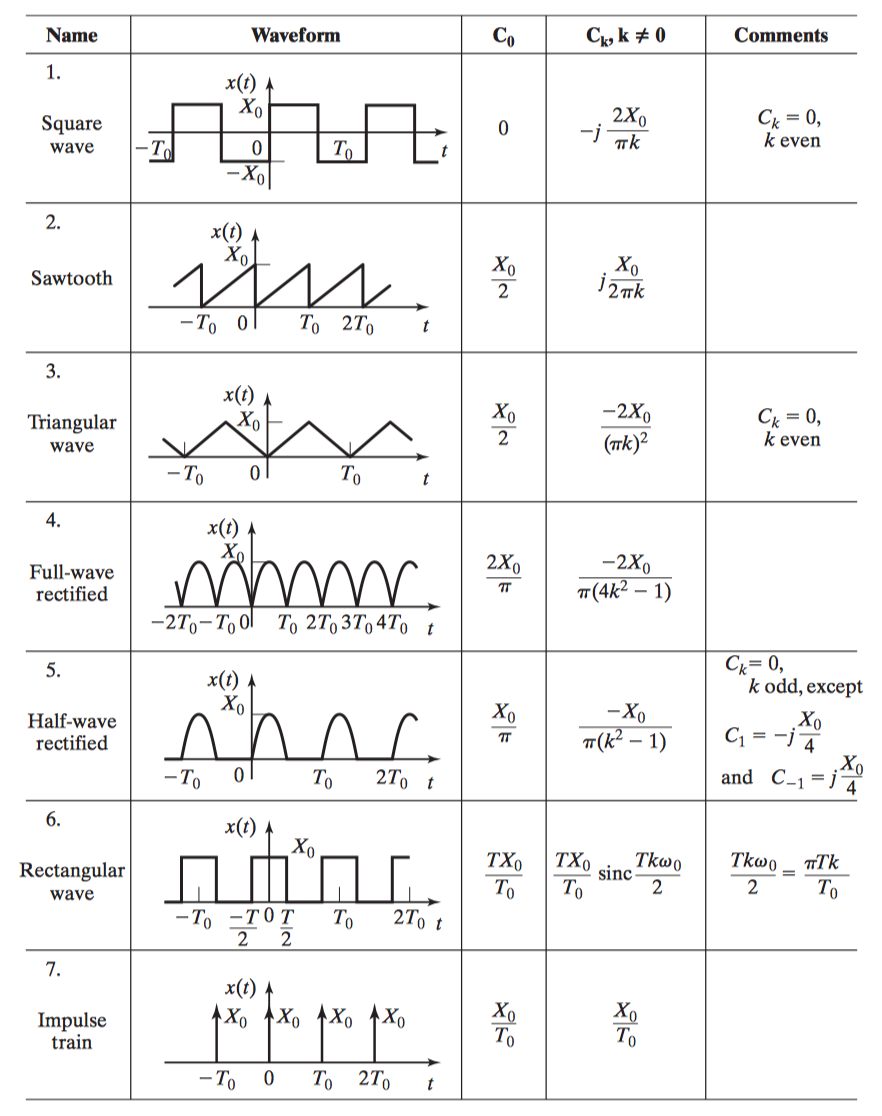
\includegraphics[width=0.95\linewidth]{1.png}
\end{minipage}
\begin{minipage}{0.48\linewidth}
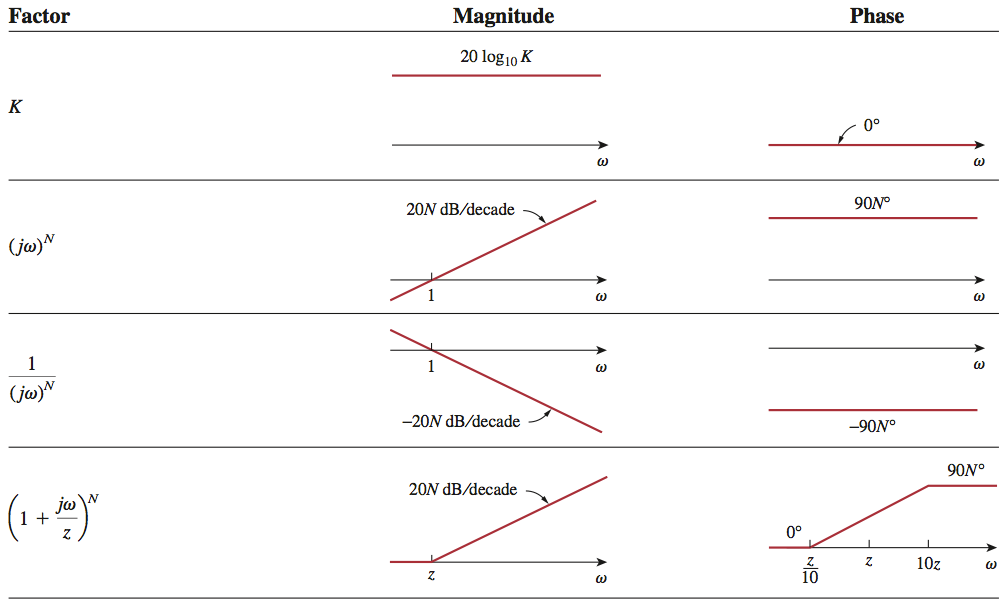
\includegraphics[width=0.95\linewidth]{2.png}
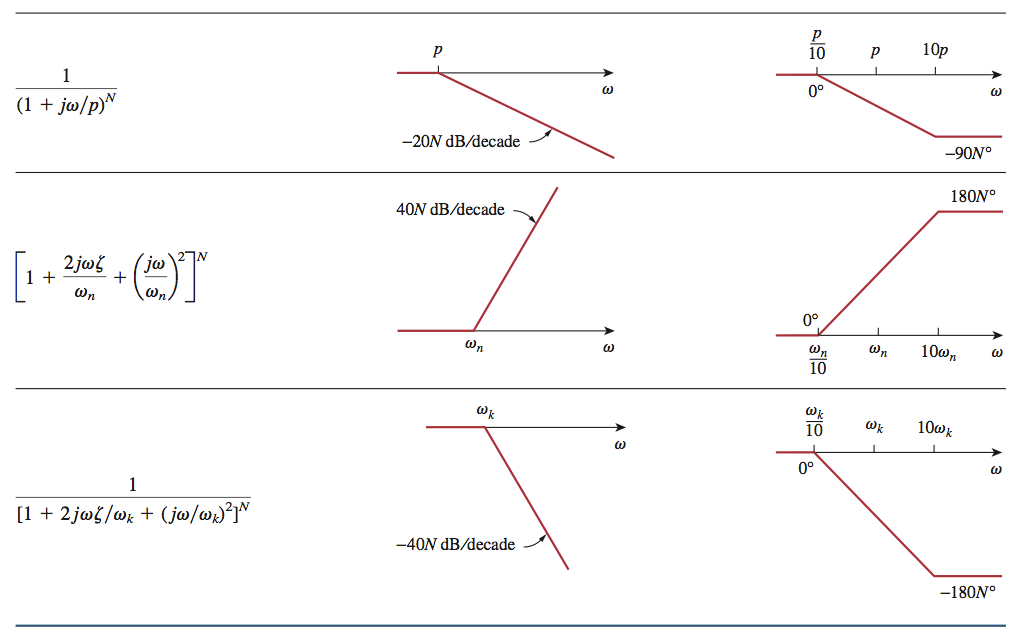
\includegraphics[width=0.95\linewidth]{3.png}
\end{minipage}

\newpage

\begin{table}[htbp]
\centering
\begin{tabular}{p{12em}<{\centering}cccc}
\hline
Property & Aperiodic Signal & Fourier transform & Aperiodic Signal & Fourier transform \\
\hline
& \\
\multicolumn{2}{c}{$\left.\begin{aligned}x(t)\\y(t)\end{aligned}\right\}\begin{aligned}&\mathrm{Period\ with\ period\ }T\ \mathrm{and}\\&\mathrm{fundamental\ frenquency\ }\omega_0=2\pi/T\end{aligned}$ }
& $\begin{aligned}a_k\\b_k\end{aligned}$ 
& $\left.\begin{aligned}x[n]\\y[n]\end{aligned}\right\}\begin{aligned}&\mathrm{Period\ with\ period\ }N\ \mathrm{and}\\&\mathrm{fundamental\ frenquency\ }\omega_0=2\pi/N\end{aligned}$ 
& $\left.\begin{aligned}X(e^{j\omega})\\Y(e^{j\omega})\end{aligned}\right\}\begin{aligned}&{\rm periodic\ with}\\&{\rm period}\ N\end{aligned}$ \\
& \\
\hdashline
& \\
Linearity & $Ax(t)+By(t)$ & $Aa_k+Bb_k$
& $Ax[n]+By[n]$ & $Aa_k+Bb_k$ \\

Time Shifting & $x(t-t_0)$ & $a_ke^{-jk\omega_0 t_0}=a_ke^{-jk(2\pi/T)t_0}$
& $x[n-n_0]$ & $a_ke^{-jk(2\pi/N)n_0}$ \\

Frequency Shifting & $e^{-jM\omega_0 t}=e^{-jM(2\pi/T) t}x(t)$ & $a_{k-M}$ 
& $e^{-jM(2\pi/N) t}x[n]$ & $a_{k-M}$ \\

Conjugation & $x^*(t)$ & $a^*_{-k}$ 
& $x^*[n]$ & $a^*_{-k}$ \\

Time Reversal & $x(-t)$ & $a_{-k}$ 
& $x[-n]$ & $a_{-k}$ \\

Time and Frequency Scaling / Time expansion & $x(\alpha t),\alpha>0$ & $a_{-k}$ 
& $x_m[n]=\left\{\begin{aligned}
& x[n/m] & \mathrm{if}\ n=\ \mathrm{multiple\ of}\ m\\
& 0 & \mathrm{if}\ n\neq\ \mathrm{multiple\ of}\ m
\end{aligned}\right.$ & $\dfrac{1}{m}a_k$\\

Periodic Convolution & $\displaystyle\int_Tx(\tau)y(t-\tau)d\tau$ & $Ta_kb_k$
& $\displaystyle\sum_{r=<N>}x[r]y[n-r]$ & $Na_kb_k$ \\

Multiplication & $x(t)y(t)$ & $\displaystyle\sum_{l=-\infty}^{+\infty}a_lb_k-l$ 
& $x[n]y[n]$ & $\displaystyle\sum_{l=<N>}a_lb_{k-l}$\\

Differentiation & $\dfrac{d}{dt}x(t)$ & $jk\omega_0a_k=jk\dfrac{2\pi}{T}a_k$
& $x[n]-x[n-1]$ & $(1-e^{-jk(2\pi/N)})a_k$ \\

Integration/Accumulation & $\displaystyle\int_{-\infty}^tx(t)dt$ & $\dfrac{1}{jk\omega_0}a_k=\dfrac{1}{jk(2\pi/T)}a_k$ 
& $\displaystyle\sum\limits_{k=-\infty}^{+\infty}x[k]$ & $\dfrac{1}{1-e^{-jk(2\pi/N)}}a_k$ \\

Conjugate Symmetry for Real Signals & $x(t)$ real & 
$\left\lbrace\begin{aligned}
&a_k=a^*_{-k} \\
&\mathfrak{Re}\{a_k\}=\mathfrak{Re}\{a_{-k}\} \\
&\mathfrak{Im}\{a_k\}=-\mathfrak{Im}\{a_{-k}\} \\
&|a_k|=|a_{-k}| \\
&\sphericalangle a_k=-\sphericalangle a_{-k} \\
\end{aligned}\right.$
& $x[n]$ real & 
$\left\lbrace\begin{aligned}
&a_k=a^*_{-k} \\
&\mathfrak{Re}\{a_k\}=\mathfrak{Re}\{a_{-k}\} \\
&\mathfrak{Im}\{a_k\}=-\mathfrak{Im}\{a_{-k}\} \\
&|a_k|=|a_{-k}| \\
&\sphericalangle a_k=-\sphericalangle a_{-k} \\
\end{aligned}\right.$\\
& \\

Symmetry for Real and Even Signals & $x(t)$ real and even & $a_k$ real and even 
& $x[n]$ real and even & $a_k$ real and even \\

Symmetry for Real and Odd Signals & $x(t)$ real and odd & $a_k$ purely imaginary and odd 
& $x[n]$ real and odd & $a_k$ purely imaginary and odd \\

Even-Odd Decomposition for Real Signals & 
$\begin{aligned}
x_e(t)&=\mathfrak{Ev}\{x(t)\} & [x(t){\rm\ real}] \\
x_o(t)&=\mathfrak{Od}\{x(t)\} & [x(t){\rm\ real}] \\
\end{aligned}$ & 
$\begin{aligned}
&\mathfrak{Re}\{a_k\} \\
&j\mathfrak{Im}\{a_k\} \\
\end{aligned}$ &
$\begin{aligned}
x_e[n]&=\mathfrak{Ev}\{x[n]\} & [x[n]{\rm\ real}] \\
x_o[n]&=\mathfrak{Od}\{x[n]\} & [x[n]{\rm\ real}] \\
\end{aligned}$ & 
$\begin{aligned}
&\mathfrak{Re}\{a_k\} \\
&j\mathfrak{Im}\{a_k\} \\
\end{aligned}$ \\
& \\
\hdashline
& \\
Parseval's Relation for Aperiodic Signals 
& \multicolumn{2}{c}{$\displaystyle\frac{1}{T}\int_T|x(t)|^2dt=\sum_{k=-\infty}^{+\infty}|a_k|^2$}
& \multicolumn{2}{c}{$\displaystyle\frac{1}{N}\sum_N|x[n]|^2=\sum_{k=<N>}|a_k|^2$} \\
\hline
\end{tabular}
\caption{Properties of Fourier Series}
\end{table}

\newpage

\begin{table}[htbp]
\centering
\begin{tabular}{p{12em}<{\centering}cccc}
\hline
Property & Aperiodic Signal & Fourier transform & Aperiodic Signal & Fourier transform \\
\hline
& \\
& $\begin{aligned}x(t)\\y(t)\end{aligned}$ 
& $\begin{aligned}X(j\omega)\\Y(j\omega)\end{aligned}$ 
& $\begin{aligned}x[n]\\y[n]\end{aligned}$ 
& $\left.\begin{aligned}X(e^{j\omega})\\Y(e^{j\omega})\end{aligned}\right\}\begin{aligned}&{\rm periodic\ with}\\&{\rm period}\ 2\pi\end{aligned}$ \\
& \\
\hdashline
& \\
Linearity & $ax(t)+by(t)$ & $aX(j\omega)+bY(j\omega)$
& $ax[n]+by[n]$ & $aX(e^{j\omega})+bY(e^{j\omega})$ \\
Time Shifting & $x(t-t_0)$ & $e^{-j\omega t_0}X(j\omega)$
& $x[n-n_0]$ & $e^{-j\omega n_0}X(e^{j\omega})$ \\
Frequency Shifting & $e^{-j\omega t_0}x(t)$ & $X(j(\omega-\omega_0))$ 
& $e^{j\omega_0n}$ & $X(e^{j(\omega-\omega_0)})$ \\
Conjugation & $x^*(t)$ & $X^*(-j\omega)$ 
& $x^*[n]$ & $X^*(e^{-j\omega})$ \\
Time Reversal & $x(-t)$ & $X(-j\omega)$ 
& $x[-n]$ & $X(e^{-j\omega})$ \\
Time and Frequency Scaling / Time expansion & $x(at)$ & $\dfrac{1}{|a|}X(\dfrac{j\omega}{a})$ 
& $x_k[n]=\left\{\begin{aligned}
& x[n/k] & \mathrm{if}\ n=\ \mathrm{multiple\ of}\ k\\
& 0 & \mathrm{if}\ n\neq\ \mathrm{multiple\ of}\ k
\end{aligned}\right.$ & $X(e^{jk\omega})$\\
Convolution & $x(t)*y(t)$ & $X(j\omega)Y(j\omega)$
& $x[n]*y[n]$ & $X(e^{j\omega})Y(e^{j\omega})$ \\
Multiplication & $x(t)y(t)$ & $\displaystyle\dfrac{1}{2\pi}\int_{-\infty}^{+\infty}X(j\omega)Y(j(\omega-\theta))d\theta$ 
& $x[n]y[n]$ & $\displaystyle\dfrac{1}{2\pi}\int_{2\pi} X(e^{j\theta})Y(e^{j(\omega-\theta)})d\theta$ \\
Differentiation in Time & $\dfrac{d}{dt}x(t)$ & $j\omega X(j\omega)$
& $x[n]-x[n-1]$ & $(1-e^{-j\omega})X(e^{j\omega})$ \\
Integration/Accumulation & $\displaystyle\int_{-\infty}^tx(t)dt$ & $\dfrac{1}{j\omega}X(j\omega)+\pi X(0)\delta(\omega)$ 
& $\displaystyle\sum\limits_{k=-\infty}^{+\infty}x[k]$ & $\dfrac{1}{1-e^{-j\omega}}X(e^{j\omega})$ \\
Differentiation in Frequency & $tx(t)$ & $j\dfrac{d}{d\omega}X(j\omega)$ 
& $nx[n]$ & $j\dfrac{dX(e^{j\omega})}{d\omega}$ \\
Conjugate Symmetry for Real Signals & $x(t)$ real & 
$\left\lbrace\begin{aligned}
&X(j\omega)=X^*(-j\omega) \\
&\mathfrak{Re}\{X(j\omega)\}=\mathfrak{Re}\{X(-j\omega)\} \\
&\mathfrak{Im}\{X(j\omega)\}=-\mathfrak{Im}\{X(-j\omega)\} \\
&|X(j\omega)|=|X(-j\omega)| \\
&\sphericalangle X(j\omega)=-\sphericalangle X(-j\omega) \\
\end{aligned}\right.$
& $x[n]$ real & 
$\left\lbrace\begin{aligned}
&X(e^{j\omega})=X^*(e^{-j\omega}) \\
&\mathfrak{Re}\{X(e^{j\omega})\}=\mathfrak{Re}\{X(e^{-j\omega})\} \\
&\mathfrak{Im}\{X(e^{j\omega})\}=-\mathfrak{Im}\{X(e^{-j\omega})\} \\
&|X(e^{j\omega})|=|X(e^{-j\omega})| \\
&\sphericalangle X(e^{j\omega})=-\sphericalangle X(e^{-j\omega}) \\
\end{aligned}\right.$\\
& \\
Symmetry for Real and Even Signals & $x(t)$ real and even & $X(j\omega)$ real and even 
& $x[n]$ real and even & $X(e^{j\omega})$ real and even \\
Symmetry for Real and Odd Signals & $x(t)$ real and odd & $X(j\omega)$ purely imaginary and odd 
& $x[n]$ real and odd & $X(e^{j\omega})$ purely imaginary and odd \\
Even-Odd Decomposition for Real Signals & 
$\begin{aligned}
x_e(t)&=\mathfrak{Ev}\{x(t)\} & [x(t){\rm\ real}] \\
x_o(t)&=\mathfrak{Od}\{x(t)\} & [x(t){\rm\ real}] \\
\end{aligned}$ & 
$\begin{aligned}
&\mathfrak{Re}\{X(j\omega)\} \\
&j\mathfrak{Im}\{X(j\omega)\} \\
\end{aligned}$ &
$\begin{aligned}
x_e[n]&=\mathfrak{Ev}\{x[n]\} & [x[n]{\rm\ real}] \\
x_o[n]&=\mathfrak{Od}\{x[n]\} & [x[n]{\rm\ real}] \\
\end{aligned}$ & 
$\begin{aligned}
&\mathfrak{Re}\{X(e^{j\omega})\} \\
&j\mathfrak{Im}\{X(e^{j\omega})\} \\
\end{aligned}$ \\
& \\
\hdashline
& \\
Parseval's Relation for Aperiodic Signals 
& \multicolumn{2}{c}{$\displaystyle\int_{-\infty}^{+\infty}|x(t)|^2dt=\dfrac{1}{2\pi}\int_{-\infty}^{+\infty}|X(j\omega)|^2d\omega$} 
& \multicolumn{2}{c}{$\displaystyle\sum\limits_{n=-\infty}^{+\infty}|x[n]|^2dt=\dfrac{1}{2\pi}\int_{2\pi}|X(e^{j\omega})|^2d\omega$} \\
\hline
\end{tabular}
\caption{Properties of Fourier Transform}
\end{table}

\newpage

\begin{table}[htbp]
\centering
\small
\begin{tabular}{p{13em}<{\centering}cp{7em}p{12em}<{\centering}p{14em}<{\centering}p{18em}}
\hline
Signal & Fourier transform & Fourier series coefficients &
Signal & Fourier transform & Fourier series coefficients \\
\hline

$\displaystyle\sum_{k=-\infty}^{+\infty}a_ke^{jk\omega_0t}$ & $\displaystyle 2\pi\sum_{k=-\infty}^{+\infty}a_k\delta(\omega-k\omega_0)$ & $a_k$ &
$\displaystyle\sum_{k=<N>)}a_ke^{jk(2n/N)n}$ & $\displaystyle 2\pi\sum_{k=-\infty}^{+\infty}a_k\delta\left(\omega-\frac{2\pi k}{N}\right)$ & $a_k$ \\

$e^{j\omega_0t}$ & $2\pi\delta(\omega-k\omega_0)$ & $\begin{aligned}&a_1=1\\&a_k=0,\rm\ otherwise\end{aligned}$ &
$e^{j\omega_0n}$ & $\displaystyle 2\pi\sum_{l=-\infty}^{+\infty}\delta(\omega-\omega_0-2\pi l)$ & $\begin{aligned}&\omega_0=\frac{2\pi m}{N}\\&a_k=\left\{\begin{aligned}1,&k=m,m\pm N,m\pm 2N,\dots\\ 0,&{\rm otherwise}\end{aligned}\right.\end{aligned}$\\

$\cos\omega_0t$ & $\pi[\delta(\omega-k\omega_0)+\delta(\omega+k\omega_0)]$ & $\begin{aligned}&a_1=a_{-1}=\frac{1}{2}\\&a_k=0,\rm\ otherwise\end{aligned}$ &
$\cos\omega_0 n$ & $\displaystyle \pi\sum_{l=-\infty}^{+\infty}\delta(\omega-\omega_0-2\pi l)+\delta(\omega+\omega_0-2\pi l)$ & $\begin{aligned}&\omega_0=\frac{2\pi m}{N}\\&a_k=\left\{\begin{aligned}\frac{1}{2},&k=\pm m,\pm m\pm N,\pm m\pm 2N,\dots\\ 0,&{\rm otherwise}\end{aligned}\right.\end{aligned}$\\

$\sin\omega_0t$ & $\dfrac{\pi}{j}\delta(\omega-k\omega_0)-\delta(\omega+k\omega_0)]$ & $\begin{aligned}&a_1=a_{-1}=\frac{1}{2j}\\&a_k=0,\rm\ otherwise\end{aligned}$ &
$\sin\omega_0 n$ & $\displaystyle \frac{\pi}{j}\sum_{l=-\infty}^{+\infty}\delta(\omega-\omega_0-2\pi l)-\delta(\omega+\omega_0-2\pi l)$ & $\begin{aligned}&\omega_0=\frac{2\pi r}{N}\\&a_k=\left\{\begin{aligned}\frac{1}{2j},&k=r,r\pm N,r\pm 2N,\dots\\-\frac{1}{2j},&k=-r,-r\pm N,-r\pm 2N,\dots\\ 0,&{\rm otherwise}\end{aligned}\right.\end{aligned}$ \\

$x(t)=1$ & $2\pi\delta(\omega)$ & $\begin{aligned}&a_0=1\\&a_k=0,\ k\neq 0\end{aligned}$ &
$x[n]=1$ & $2\displaystyle\pi\sum_{l=-\infty}^{+\infty}\delta(\omega-2\pi l)$ & $a_k=\left\{\begin{aligned}&1,&k=0,\pm N,\pm 2N\\&0,&\rm otherwise\ k\neq 0\end{aligned}\right.$ \\

$\begin{aligned}
&x(t)=\left\{\begin{aligned}&1,&|t|<T_1\\&0,&T_1<|t|\leqslant\frac{T}{2}\end{aligned}\right.\\
&x(t+T)=x(t)
\end{aligned}$ & $\displaystyle \sum_{k=-\infty}^{+\infty}\frac{2\sin k\omega_0T_1}{k}\delta(\omega-\omega_0)$ & $\displaystyle\frac{\sin k\omega_0T_1}{k\pi}$ & 

$\begin{aligned}
&x[n]=\left\{\begin{aligned}&1,&|n|\leqslant N_1\\&0,&N_1<|n|\leqslant N/2\end{aligned}\right.\\
&x[n+N]=x[n]
\end{aligned}$ & $\displaystyle 2\pi\sum_{k=-\infty}^{+\infty}a_k\delta\left(\omega-\frac{2\pi k}{N}\right)$ & $\begin{aligned}&a_k=\frac{\sin[(2\pi k/N)(N_1+\frac12)]}{N\sin[2\pi k/2N]},k\neq 0,\pm N,\pm 2N\\&a_k=\frac{2N_1+1}{N},k=0,\pm N,\pm 2N\end{aligned}$ \\

$\displaystyle\sum_{n=-\infty}^{+\infty}\delta(t-nT)$ & $\displaystyle\frac{2\pi}{T}\sum_{n=-\infty}^{+\infty}\delta\left(\omega-\frac{2\pi k}{T}\right)$ & $a_k=\dfrac{1}{T}$ for all $k$ & 
$\displaystyle\sum_{n=-\infty}^{+\infty}\delta[n-kN]$ & $\displaystyle\frac{2\pi}{N}\sum_{n=-\infty}^{+\infty}\delta\left(\omega-\frac{2\pi k}{N}\right)$ & $a_k=\dfrac{1}{T}$ for all $k$ \\

$x(t)\left\{\begin{aligned}&1,&|t|<T_1\\&0,&|t|>T_1\end{aligned}\right.$ & $\dfrac{2\sin\omega T_1}{\omega}$ & --- &
$x[n]\left\{\begin{aligned}&1,&|n|\leqslant N\\&0,&|n|>N\end{aligned}\right.$ & $\dfrac{\sin[\omega(N_1+\frac{1}{2})]}{\sin(\omega/2)}$ & --- \\

$\dfrac{\sin Wt}{\pi t}$ & $X(j\omega)=\left\{\begin{aligned}&1,&|\omega|<W\\&0,&|\omega|>W\end{aligned}\right.$ & --- &
$\dfrac{\sin Wn}{\pi n}=\dfrac{W}{\pi}{\rm sinc}\left(\dfrac{Wn}{\pi}\right)$ & $X(\omega)=\left\{\begin{aligned}&1,&0<|\omega|<W\\&0,&W<|\omega|<\pi\end{aligned}\right.$ & --- \\

$\delta(t)$ & $1$ & --- &
$\delta[n]$ & $1$ & --- \\

$u(t)$ & $\dfrac{1}{j\omega}+\pi\delta(\omega)$ & --- &
$u[n]$ & $\displaystyle\dfrac{1}{1-e^{-j\omega}}+\sum_{k=-\infty}^{+\infty}\pi\delta(\omega-2\pi k)$ & --- \\

$\delta(t-t_0)$ & $e^{-j\omega t_0}$ & --- &
$\delta[n-n_0]$ & $e^{-j\omega n_0}$ & --- \\

$e^{-at}u(t),\mathfrak{Re}\{a\}>0$ & $\dfrac{1}{a+j\omega}$ & --- &
$a^nu[n],|a|<1$ & $\dfrac{1}{1-ae^{-j\omega}}$ & --- \\

$te^{-at}u(t),\mathfrak{Re}\{a\}>0$ & $\dfrac{1}{(a+j\omega)^2}$ & --- &
$(n+1)a^nu[n],|a|<1$ & $\dfrac{1}{(1-ae^{-j\omega})^2}$ & --- \\

$\dfrac{t^{n-1}}{(n-1)!}e^{-at}u(t),\mathfrak{Re}\{a\}>0$ & $\dfrac{1}{(a+j\omega)^n}$ & --- &
$\dfrac{(n+r-1)!}{n!(r-1)!}a^nu[n],|a|<1$ & $\dfrac{1}{(1-ae^{-j\omega})^n}$ & --- \\

\hline
\end{tabular}
\caption{Basic Fourier Transform Pairs}
\end{table}



\end{document}
